\subsection{Contexto de Simetr\'ia}
\begin{frame}[t]
\frametitle{\secname}
\framesubtitle{Contexto de Simetr\'ia}
\vspace{-0.5cm}
\begin{tikzpicture}[remember picture, overlay]
\node<1->[anchor = north west, text width =0.7\textwidth, yshift = -0.75cm](txt) at (current page.north west) {
	\begin{tcolorbox}[enhanced,title =Contexto de Simetr\'ia,
	left=1mm,
	top=1mm,
	bottom=1mm,
	right=1mm,
	width =\textwidth,
	height=0.28\textheight,
	boxsep = 0cm,
	coltitle=blue,
	attach boxed title to top center={yshift=-2mm,yshifttext=-1mm},
	boxed title style={colframe=blue,
		colback=gc!90}]
	\begin{itemize}
	\item<1-> Simetr\'ia es un cambio sin cambio.
	\item<2-> Transformaciones u operaciones que no alteran un ``objeto''
	\item<3-> En f\'isica la formalidad de la simetr\'ia la otorga la \textcolor{magenta}{teoria de grupos}
	\end{itemize}
	\end{tcolorbox}	
};

\node<1->[anchor=north east,xshift=-20mm,yshift=-9mm] (i1) at (current page.north east){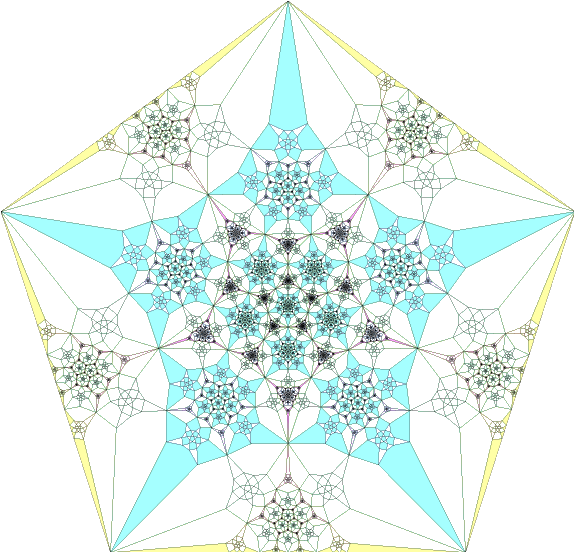
\includegraphics[width=0.33\textwidth]{../beamer-figures/physical-model/BigPlatoBig.png}};
\node<2-3>[anchor=north west,inner sep=0mm,xshift=2mm,yshift=2mm](sym1) at (txt.south west){\animategraphics[autoplay,loop,width=0.22\textwidth,]{20}{beamer-figures/physical-model/sym1}{}{}};
\node<2-3>[anchor=north west,inner sep=0mm,xshift=2mm](sym2) at (sym1.north east){\animategraphics[autoplay,loop,width=0.22\textwidth,]{20}{beamer-figures/physical-model/sym2}{}{}};
\node<2-3>[anchor=north west,inner sep=0mm,xshift=2mm,yshift=-3.5mm](sym3) at (sym2.north east){\animategraphics[autoplay,loop,width=0.22\textwidth,]{20}{beamer-figures/physical-model/sym3}{}{}};
\node<2-3>[anchor=north west,inner sep=0mm,xshift=2mm](sym4) at (sym3.north east){\animategraphics[autoplay,loop,width=0.22\textwidth,]{20}{beamer-figures/physical-model/sym4}{}{}};

\node<2-3>[anchor=north,inner sep=0mm,xshift=0mm](sym5) at (sym1.south){\animategraphics[autoplay,loop,width=0.22\textwidth,]{20}{beamer-figures/physical-model/sym5}{}{}};
\node<2-3>[anchor=north,inner sep=0mm,xshift=0mm](sym6) at (sym2.south){\animategraphics[autoplay,loop,width=0.22\textwidth,]{20}{beamer-figures/physical-model/sym6}{}{}};
\node<2-3>[anchor=north,inner sep=0mm,xshift=0mm,yshift=-3mm](sym7) at (sym3.south){\animategraphics[autoplay,loop,width=0.22\textwidth,]{20}{beamer-figures/physical-model/sym7}{}{}};
\node<2-3>[anchor=north,inner sep=0mm,xshift=0mm](sym8) at (sym4.south){\animategraphics[autoplay,loop,width=0.22\textwidth,]{20}{beamer-figures/physical-model/sym8}{}{}};

\node<2-3>[anchor=south west, text width=\textwidth,scale=0.7,text=gc] at (current page.south west){Attribution: symotter.org/gallery};


\end{tikzpicture}
\end{frame}
	
	
\subsection{Simetr\'ia y Estructura de Bandas}
\begin{frame}[t]
\frametitle{\secname}
\framesubtitle{\subsecname}
\vspace{-0.5cm}
\begin{tikzpicture}[remember picture, overlay]
\node<1->[anchor = north west, text width =0.65\textwidth, yshift = -0.75cm](txt) at (current page.north west) {
	\begin{tcolorbox}[enhanced,title =\subsecname,
	left=1mm,
	top=1mm,
	bottom=1mm,
	right=1mm,
	width =\textwidth,
	height=0.2\textheight,
	boxsep = 0cm,
	coltitle=blue,
	attach boxed title to top center={yshift=-2mm,yshifttext=-1mm},
	boxed title style={colframe=blue,
		colback=gc!90}]
	\begin{itemize}
	\item<1-> Simetr\'ia ``Macroscopica''.
	\item<2-> Simetr\'ia ``Microscopica''.\\ \textcolor{red}{\emph{La s\'imetria de un sistema define las funciones base para obteener la Estructura de Bandas}}
	
	\end{itemize}
	\end{tcolorbox}	
};

\node<1>[anchor=north west,inner sep=0mm,xshift=-5mm,yshift=5mm](sym1) at (txt.north east){\animategraphics[autoplay,loop,width=0.4\textwidth]{10}{beamer-figures/physical-model/sym9}{}{}};
\node<2->[anchor=north west,inner sep=0mm,xshift=1mm,yshift=-3mm] at  (txt.north east) {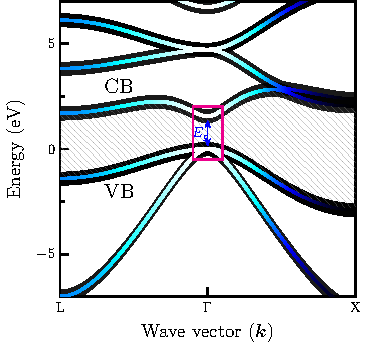
\includegraphics[width=0.35\textwidth,trim={0 0 0cm 0}]{../../figures/chapter-1/bands/build-ruco/bands01-beamer}};
\node<2->[anchor=south west,xshift=0mm,yshift=0mm] (i2) at (current page.south west){\includegraphics[width=\textwidth]{../../figures/chapter-2/symmetry/out/sym-0}};

\end{tikzpicture}
\end{frame}
	
	